% Options for packages loaded elsewhere
\PassOptionsToPackage{unicode}{hyperref}
\PassOptionsToPackage{hyphens}{url}
%
\documentclass[
  man]{apa6}
\usepackage{amsmath,amssymb}
\usepackage{lmodern}
\usepackage{iftex}
\ifPDFTeX
  \usepackage[T1]{fontenc}
  \usepackage[utf8]{inputenc}
  \usepackage{textcomp} % provide euro and other symbols
\else % if luatex or xetex
  \usepackage{unicode-math}
  \defaultfontfeatures{Scale=MatchLowercase}
  \defaultfontfeatures[\rmfamily]{Ligatures=TeX,Scale=1}
\fi
% Use upquote if available, for straight quotes in verbatim environments
\IfFileExists{upquote.sty}{\usepackage{upquote}}{}
\IfFileExists{microtype.sty}{% use microtype if available
  \usepackage[]{microtype}
  \UseMicrotypeSet[protrusion]{basicmath} % disable protrusion for tt fonts
}{}
\makeatletter
\@ifundefined{KOMAClassName}{% if non-KOMA class
  \IfFileExists{parskip.sty}{%
    \usepackage{parskip}
  }{% else
    \setlength{\parindent}{0pt}
    \setlength{\parskip}{6pt plus 2pt minus 1pt}}
}{% if KOMA class
  \KOMAoptions{parskip=half}}
\makeatother
\usepackage{xcolor}
\IfFileExists{xurl.sty}{\usepackage{xurl}}{} % add URL line breaks if available
\IfFileExists{bookmark.sty}{\usepackage{bookmark}}{\usepackage{hyperref}}
\hypersetup{
  pdftitle={The Structure of Chaos: An Empirical Comparison of Fractal Physiology Complexity Indices using NeuroKit2},
  pdfauthor={Dominique Makowski1, An Shu Te1, Tam Pham1, Zen J. Lau1, \& S.H. Annabel Chen1},
  pdflang={en-EN},
  pdfkeywords={chaos, complexity, fractal, physiology, noise},
  hidelinks,
  pdfcreator={LaTeX via pandoc}}
\urlstyle{same} % disable monospaced font for URLs
\usepackage{graphicx}
\makeatletter
\def\maxwidth{\ifdim\Gin@nat@width>\linewidth\linewidth\else\Gin@nat@width\fi}
\def\maxheight{\ifdim\Gin@nat@height>\textheight\textheight\else\Gin@nat@height\fi}
\makeatother
% Scale images if necessary, so that they will not overflow the page
% margins by default, and it is still possible to overwrite the defaults
% using explicit options in \includegraphics[width, height, ...]{}
\setkeys{Gin}{width=\maxwidth,height=\maxheight,keepaspectratio}
% Set default figure placement to htbp
\makeatletter
\def\fps@figure{htbp}
\makeatother
\setlength{\emergencystretch}{3em} % prevent overfull lines
\providecommand{\tightlist}{%
  \setlength{\itemsep}{0pt}\setlength{\parskip}{0pt}}
\setcounter{secnumdepth}{-\maxdimen} % remove section numbering
% Make \paragraph and \subparagraph free-standing
\ifx\paragraph\undefined\else
  \let\oldparagraph\paragraph
  \renewcommand{\paragraph}[1]{\oldparagraph{#1}\mbox{}}
\fi
\ifx\subparagraph\undefined\else
  \let\oldsubparagraph\subparagraph
  \renewcommand{\subparagraph}[1]{\oldsubparagraph{#1}\mbox{}}
\fi
\newlength{\cslhangindent}
\setlength{\cslhangindent}{1.5em}
\newlength{\csllabelwidth}
\setlength{\csllabelwidth}{3em}
\newlength{\cslentryspacingunit} % times entry-spacing
\setlength{\cslentryspacingunit}{\parskip}
\newenvironment{CSLReferences}[2] % #1 hanging-ident, #2 entry spacing
 {% don't indent paragraphs
  \setlength{\parindent}{0pt}
  % turn on hanging indent if param 1 is 1
  \ifodd #1
  \let\oldpar\par
  \def\par{\hangindent=\cslhangindent\oldpar}
  \fi
  % set entry spacing
  \setlength{\parskip}{#2\cslentryspacingunit}
 }%
 {}
\usepackage{calc}
\newcommand{\CSLBlock}[1]{#1\hfill\break}
\newcommand{\CSLLeftMargin}[1]{\parbox[t]{\csllabelwidth}{#1}}
\newcommand{\CSLRightInline}[1]{\parbox[t]{\linewidth - \csllabelwidth}{#1}\break}
\newcommand{\CSLIndent}[1]{\hspace{\cslhangindent}#1}
\ifLuaTeX
\usepackage[bidi=basic]{babel}
\else
\usepackage[bidi=default]{babel}
\fi
\babelprovide[main,import]{english}
% get rid of language-specific shorthands (see #6817):
\let\LanguageShortHands\languageshorthands
\def\languageshorthands#1{}
% Manuscript styling
\usepackage{upgreek}
\captionsetup{font=singlespacing,justification=justified}

% Table formatting
\usepackage{longtable}
\usepackage{lscape}
% \usepackage[counterclockwise]{rotating}   % Landscape page setup for large tables
\usepackage{multirow}		% Table styling
\usepackage{tabularx}		% Control Column width
\usepackage[flushleft]{threeparttable}	% Allows for three part tables with a specified notes section
\usepackage{threeparttablex}            % Lets threeparttable work with longtable

% Create new environments so endfloat can handle them
% \newenvironment{ltable}
%   {\begin{landscape}\centering\begin{threeparttable}}
%   {\end{threeparttable}\end{landscape}}
\newenvironment{lltable}{\begin{landscape}\centering\begin{ThreePartTable}}{\end{ThreePartTable}\end{landscape}}

% Enables adjusting longtable caption width to table width
% Solution found at http://golatex.de/longtable-mit-caption-so-breit-wie-die-tabelle-t15767.html
\makeatletter
\newcommand\LastLTentrywidth{1em}
\newlength\longtablewidth
\setlength{\longtablewidth}{1in}
\newcommand{\getlongtablewidth}{\begingroup \ifcsname LT@\roman{LT@tables}\endcsname \global\longtablewidth=0pt \renewcommand{\LT@entry}[2]{\global\advance\longtablewidth by ##2\relax\gdef\LastLTentrywidth{##2}}\@nameuse{LT@\roman{LT@tables}} \fi \endgroup}

% \setlength{\parindent}{0.5in}
% \setlength{\parskip}{0pt plus 0pt minus 0pt}

% Overwrite redefinition of paragraph and subparagraph by the default LaTeX template
% See https://github.com/crsh/papaja/issues/292
\makeatletter
\renewcommand{\paragraph}{\@startsection{paragraph}{4}{\parindent}%
  {0\baselineskip \@plus 0.2ex \@minus 0.2ex}%
  {-1em}%
  {\normalfont\normalsize\bfseries\itshape\typesectitle}}

\renewcommand{\subparagraph}[1]{\@startsection{subparagraph}{5}{1em}%
  {0\baselineskip \@plus 0.2ex \@minus 0.2ex}%
  {-\z@\relax}%
  {\normalfont\normalsize\itshape\hspace{\parindent}{#1}\textit{\addperi}}{\relax}}
\makeatother

% \usepackage{etoolbox}
\makeatletter
\patchcmd{\HyOrg@maketitle}
  {\section{\normalfont\normalsize\abstractname}}
  {\section*{\normalfont\normalsize\abstractname}}
  {}{\typeout{Failed to patch abstract.}}
\patchcmd{\HyOrg@maketitle}
  {\section{\protect\normalfont{\@title}}}
  {\section*{\protect\normalfont{\@title}}}
  {}{\typeout{Failed to patch title.}}
\makeatother

\usepackage{xpatch}
\makeatletter
\xapptocmd\appendix
  {\xapptocmd\section
    {\addcontentsline{toc}{section}{\appendixname\ifoneappendix\else~\theappendix\fi\\: #1}}
    {}{\InnerPatchFailed}%
  }
{}{\PatchFailed}
\keywords{chaos, complexity, fractal, physiology, noise\newline\indent Word count: X}
\DeclareDelayedFloatFlavor{ThreePartTable}{table}
\DeclareDelayedFloatFlavor{lltable}{table}
\DeclareDelayedFloatFlavor*{longtable}{table}
\makeatletter
\renewcommand{\efloat@iwrite}[1]{\immediate\expandafter\protected@write\csname efloat@post#1\endcsname{}}
\makeatother
\usepackage{lineno}

\linenumbers
\usepackage{csquotes}
\usepackage[titles]{tocloft}
\cftpagenumbersoff{figure}
\renewcommand{\cftfigpresnum}{\itshape\figurename\enspace}
\renewcommand{\cftfigaftersnum}{.\space}
\setlength{\cftfigindent}{0pt}
\setlength{\cftafterloftitleskip}{0pt}
\settowidth{\cftfignumwidth}{Figure 10.\qquad}
\usepackage[labelfont=bf, font={color=gray,small}]{caption}
\ifLuaTeX
  \usepackage{selnolig}  % disable illegal ligatures
\fi

\title{\textbf{The Structure of Chaos: An Empirical Comparison of Fractal Physiology Complexity Indices using NeuroKit2}}
\author{Dominique Makowski\textsuperscript{1}, An Shu Te\textsuperscript{1}, Tam Pham\textsuperscript{1}, Zen J. Lau\textsuperscript{1}, \& S.H. Annabel Chen\textsuperscript{1}}
\date{}


\shorttitle{Structure of Chaos}

\authornote{

The authors made the following contributions. Dominique Makowski: Conceptualization, Data curation, Formal Analysis, Funding acquisition, Investigation, Methodology, Project administration, Resources, Software, Supervision, Validation, Visualization, Writing -- original draft; An Shu Te: Software, Project administration, Writing -- review \& editing; Tam Pham: Software, Writing -- review \& editing; Zen J. Lau: Software, Writing -- review \& editing; S.H. Annabel Chen: Project administration, Writing -- review \& editing.

Correspondence concerning this article should be addressed to Dominique Makowski, HSS 04-18, 48 Nanyang Avenue, Singapore. E-mail: \href{mailto:dmakowski@ntu.edu.sg}{\nolinkurl{dmakowski@ntu.edu.sg}}

}

\affiliation{\vspace{0.5cm}\textsuperscript{1} Nanyang Technological University}

\abstract{%
Complexity quantification, such as entropy, information and fractal dimension indices, are gaining a renewed traction in psychopsyiology, as new measures with promising qualities emerge from the computational and mathematical advances. Unfortunately, few studies compare the relationship and objective performance of the plethora of existing indices, in turn hindering reproducibility, replicability, and clarity in the field. In this study, we systematically compared 125 indices of complexity by their computational weight, their representativeness of a multidimensional space of latent dimensions, and empirical proximity with other indices. We propose that the selection of a few indices, such as \ldots, might offer a complimentary choice in regards to the quantification of the complexity of a time series.
}



\begin{document}
\maketitle

\hypertarget{introduction}{%
\section{Introduction}\label{introduction}}

Complexity is an umbrella term for concepts derived from information theory, chaos theory, and fractal mathematics, used to quantify unpredictability, entropy, and/or randomness. Using these tools to characterize signals (a subfield commonly referred to as ``fractal physiology,'' Bassingthwaighte et al., 2013) has shown promising results in physiology in the assessment and diagnostic of the state and health of living systems Ehlers (1995).

There has been a large and accelerating increase in the number of complexity indices in the past few decades. These new procedures are usually mathematically well-defined and theoretically promising. However, few empirical evidence exist to understand their differences and similarities. Moreover, some can be very expensive in terms of computation power and thus, time, which can become an issue in some applications such as high sampling-rate techniques (e.g., M/EEG) or real-time settings (brain-computer interface). As such, having a general view depicting the relationship between the indices with information about their computation time would be useful, for instance to guide the indices selection in settings where time or computational power is limited.

One of the contributing factor of this lack of empirical comparison is the lack of free, open-source, unified, and easy to use software for computing various complexity indices. Indeed, most of them are described mathematically in journal articles, and reusable code is seldom made available, which limits their further application and validation. \emph{NeuroKit2} (Makowski et al., 2021) is a Python package for physiological signal processing that aims at providing the most comprehensive, accurate and fast pure Python implementations of complexity indices.

Leveraging this tool, the goal of this study is to empirically compare a vast number of complexity indices, inspect how they relate to one another, and extract some recommendations for indices selection, based on their added-value and computational efficiency. Using \emph{NeuroKit2}, we will compute more than a hundred complexity indices on various types of signals, with varying degrees of noise. We will then project the results on a latent space through factor analysis, and report the most interesting indices in regards to their representation of the latent dimensions.

\hypertarget{methods}{%
\subsection{Methods}\label{methods}}

\begin{figure}
\centering
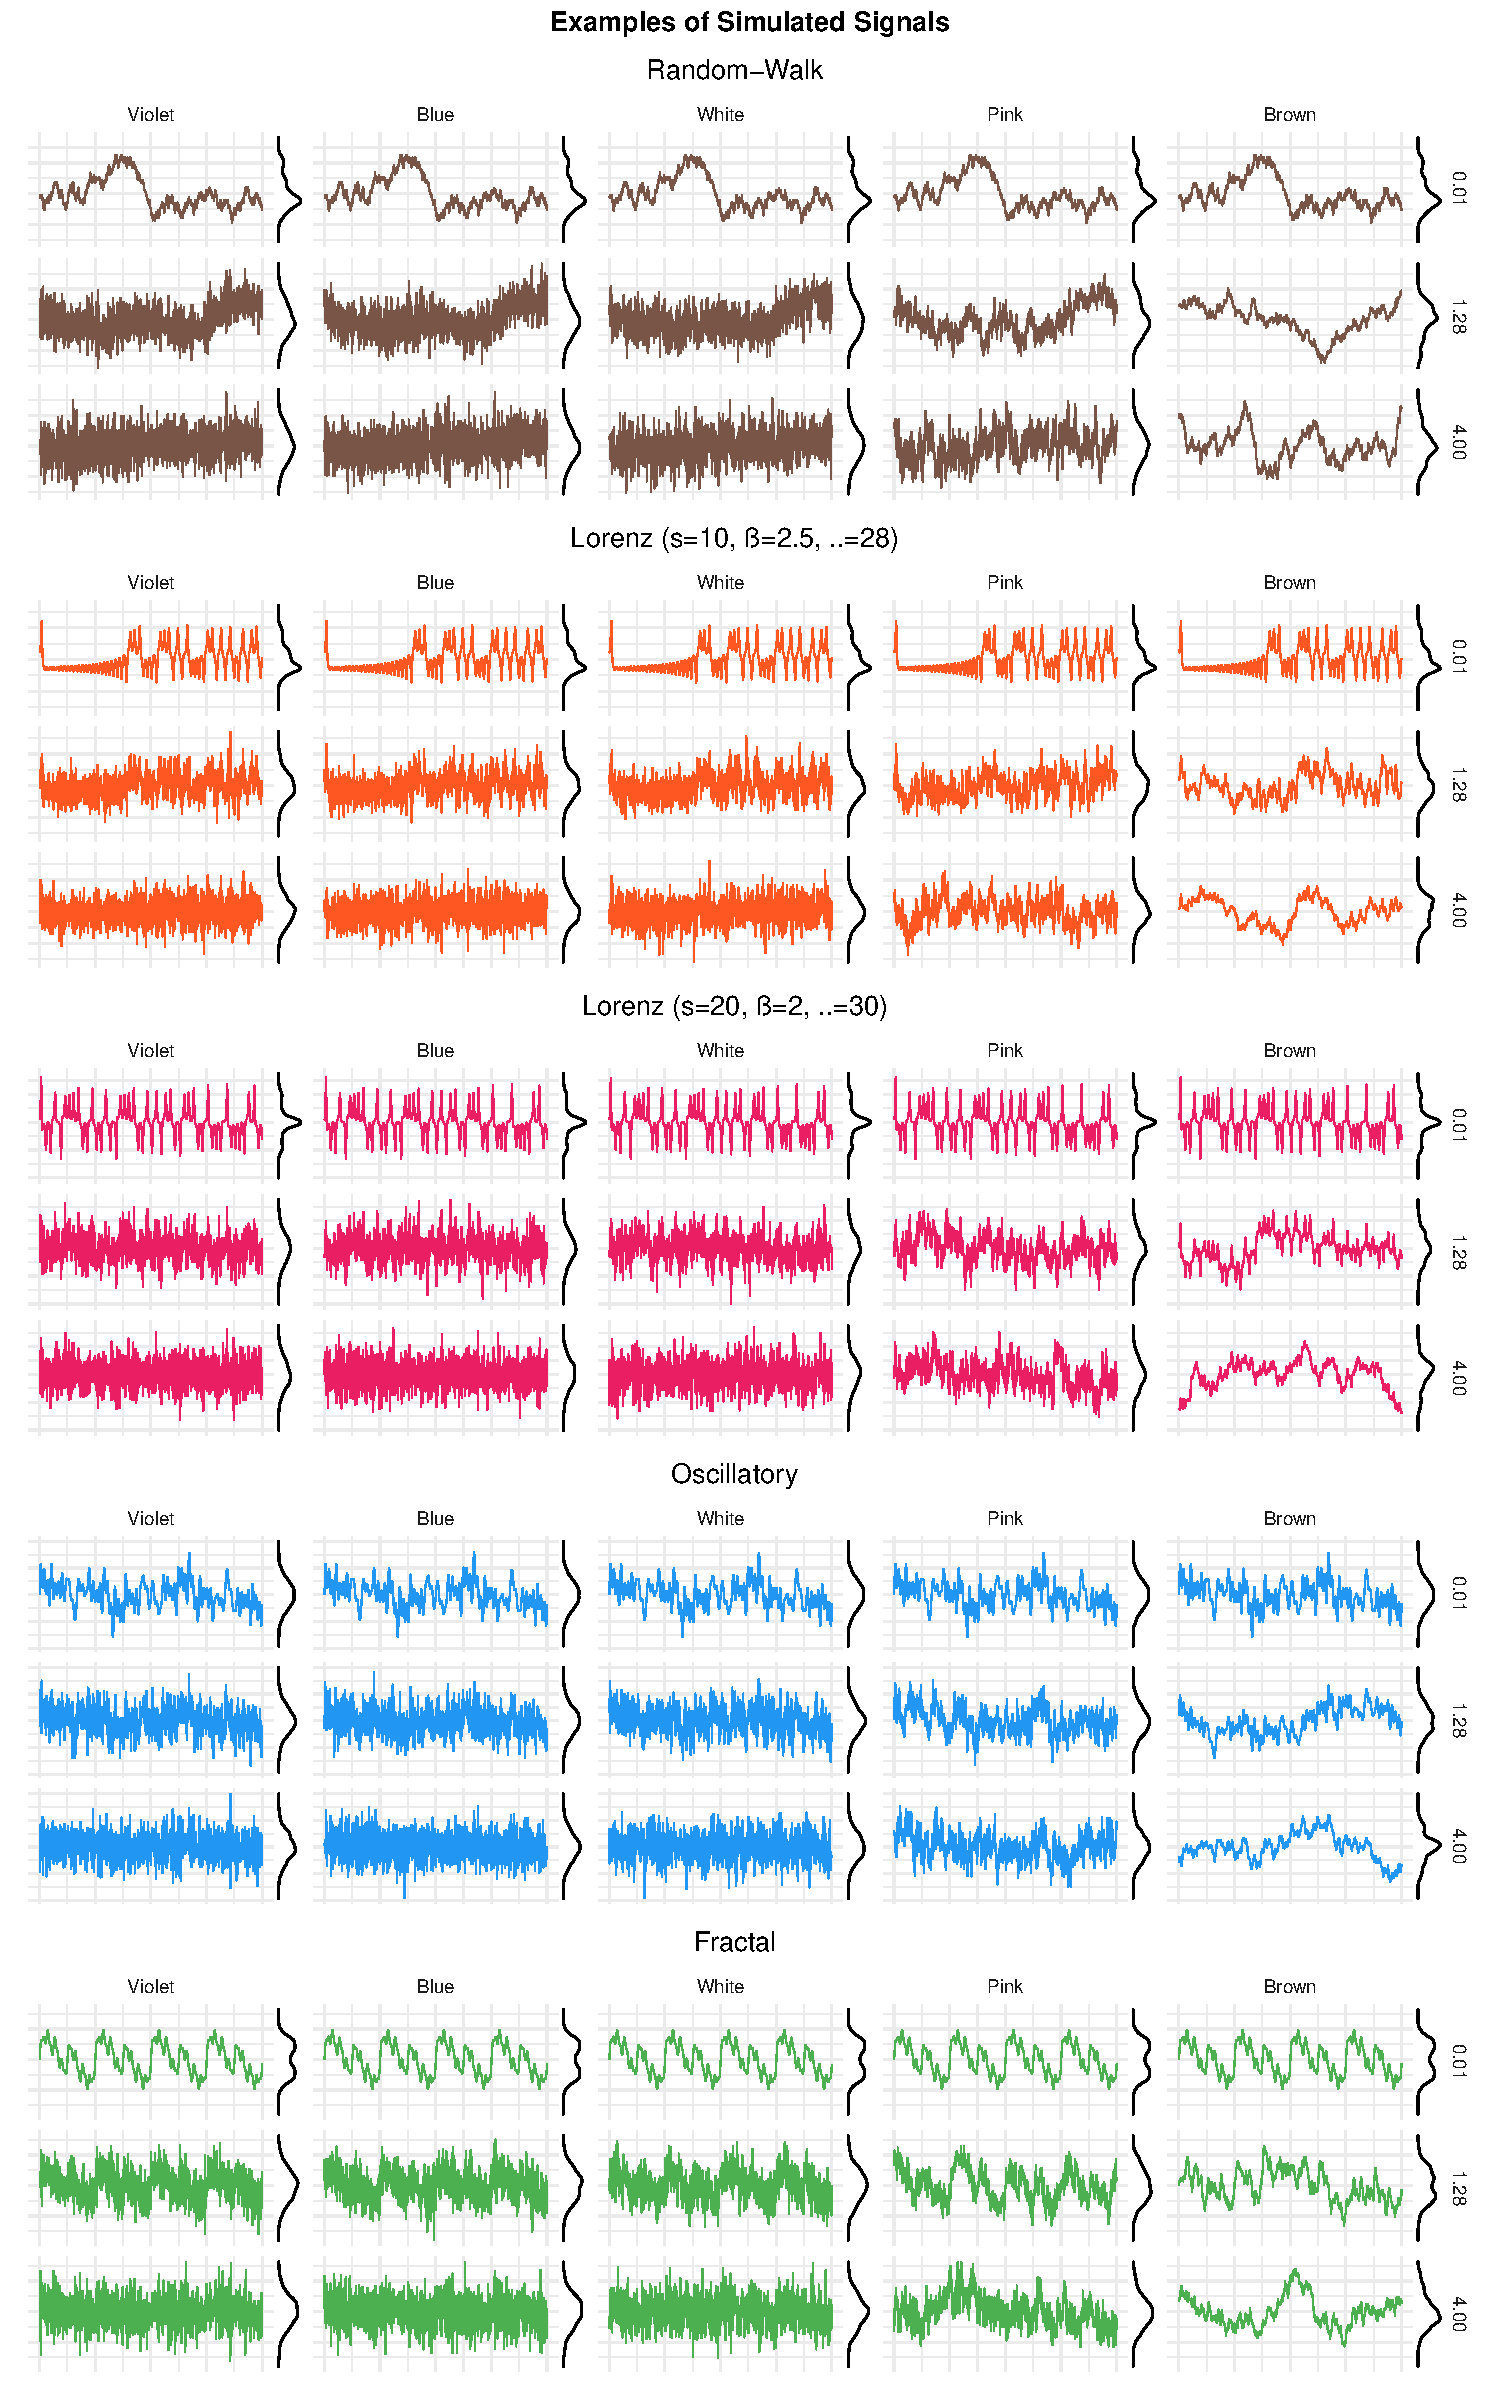
\includegraphics{manuscript_files/figure-latex/signals-1.pdf}
\caption{\label{fig:signals}Different types of simulated signals, to which was added 5 types of noise (violet, blue, white, pink, and brown) with different intensities. For each signal type, the first row shows the signal with a minimal amount of noise, and the last with a maximal amount of noise. We can see that adding Brown noise turns the signal into a Random-walk (i.e., a Brownian motion).}
\end{figure}

The script to generate the data can be found at \textbf{github.com/neuropsychology/NeuroKit/studies/complexity\_benchmark}

We started by generating 5 types of signals, one random-walk, two oscillatory signals made (one made of harmonic frequencies that results in a self-repeating - fractal-like - signal), and two complex signals derived from Lorenz systems (with parameters (\(\sigma = 10, \beta = 2.5, \rho = 28\)); and (\(\sigma = 20, \beta = 2, \rho = 30\)), respectively). Each of this signal was iteratively generated at \ldots{} different lengths (). The resulting vectors were standardized and each were added 5 types of \((1/f)^\beta\) noise (namely violet \(\beta=-2\), blue \(\beta=-1\), white \(\beta=0\), pink \(\beta=1\), and brown \(\beta=2\) noise). Each noise type was added at 48 different intensities (linearly ranging from 0.1 to 4). Examples of generated signals are presented in \textbf{Figure 1}.

The combination of these parameters resulted in a total of 6000 signal iterations. For each of them, we computed 128 complexity indices, and additionally basic metric such as the standard deviation (\emph{SD}), the \emph{length} of the signal and its dominant \emph{frequency}. The parameters used (such as the time-delay \(\tau\) or the embedding dimension) are documented in the data generation script. For a complete description of the various indices included, please refer to NeuroKit's documentation (\url{https://neuropsychology.github.io/NeuroKit}).

\hypertarget{results}{%
\subsection{Results}\label{results}}

The data analysis script, the data and the code for the figures is fully available at \textbf{ADD LINK}. The analysis was performed in R using the \emph{easystats} collection of packages (Lüdecke et al., 2021; Lüdecke et al., 2020; Makowski et al., 2020/2022, 2020).

\hypertarget{computation-time}{%
\subsubsection{Computation Time}\label{computation-time}}

Despite the relative shortness of the signals considered (a few thousand points at most), the fully-parallelized data generation script took 12h to run on a 48-cores machine. After summarizing and sorting the indices by computation time, the most striking feature are the orders of magnitude of difference between the fastest and slowest indices. Some of them are also particularly sensitive to the data length, a property which combined with computational expensiveness leads to indices being 100,000 slower to compute than other basic metrics.

Multiscale indices are among the slowest, due to their iterative nature (a given index is computed multiple times on coarse-grained subseries of the signal). Indices related to Recurrence Quantification Analysis (RQA) are also relatively slow and don't scale well with signal length.

For the subsequent analyses, we removed statistically redundant indices, such as \emph{PowEn} (identical to \emph{SD}), \emph{CREn (100)} (identical to \emph{CREn (10)}), and \emph{FuzzyRCMSEn} (identical to \emph{RCMSEn}).

\hypertarget{correlation}{%
\subsubsection{Correlation}\label{correlation}}

\begin{figure}
\centering
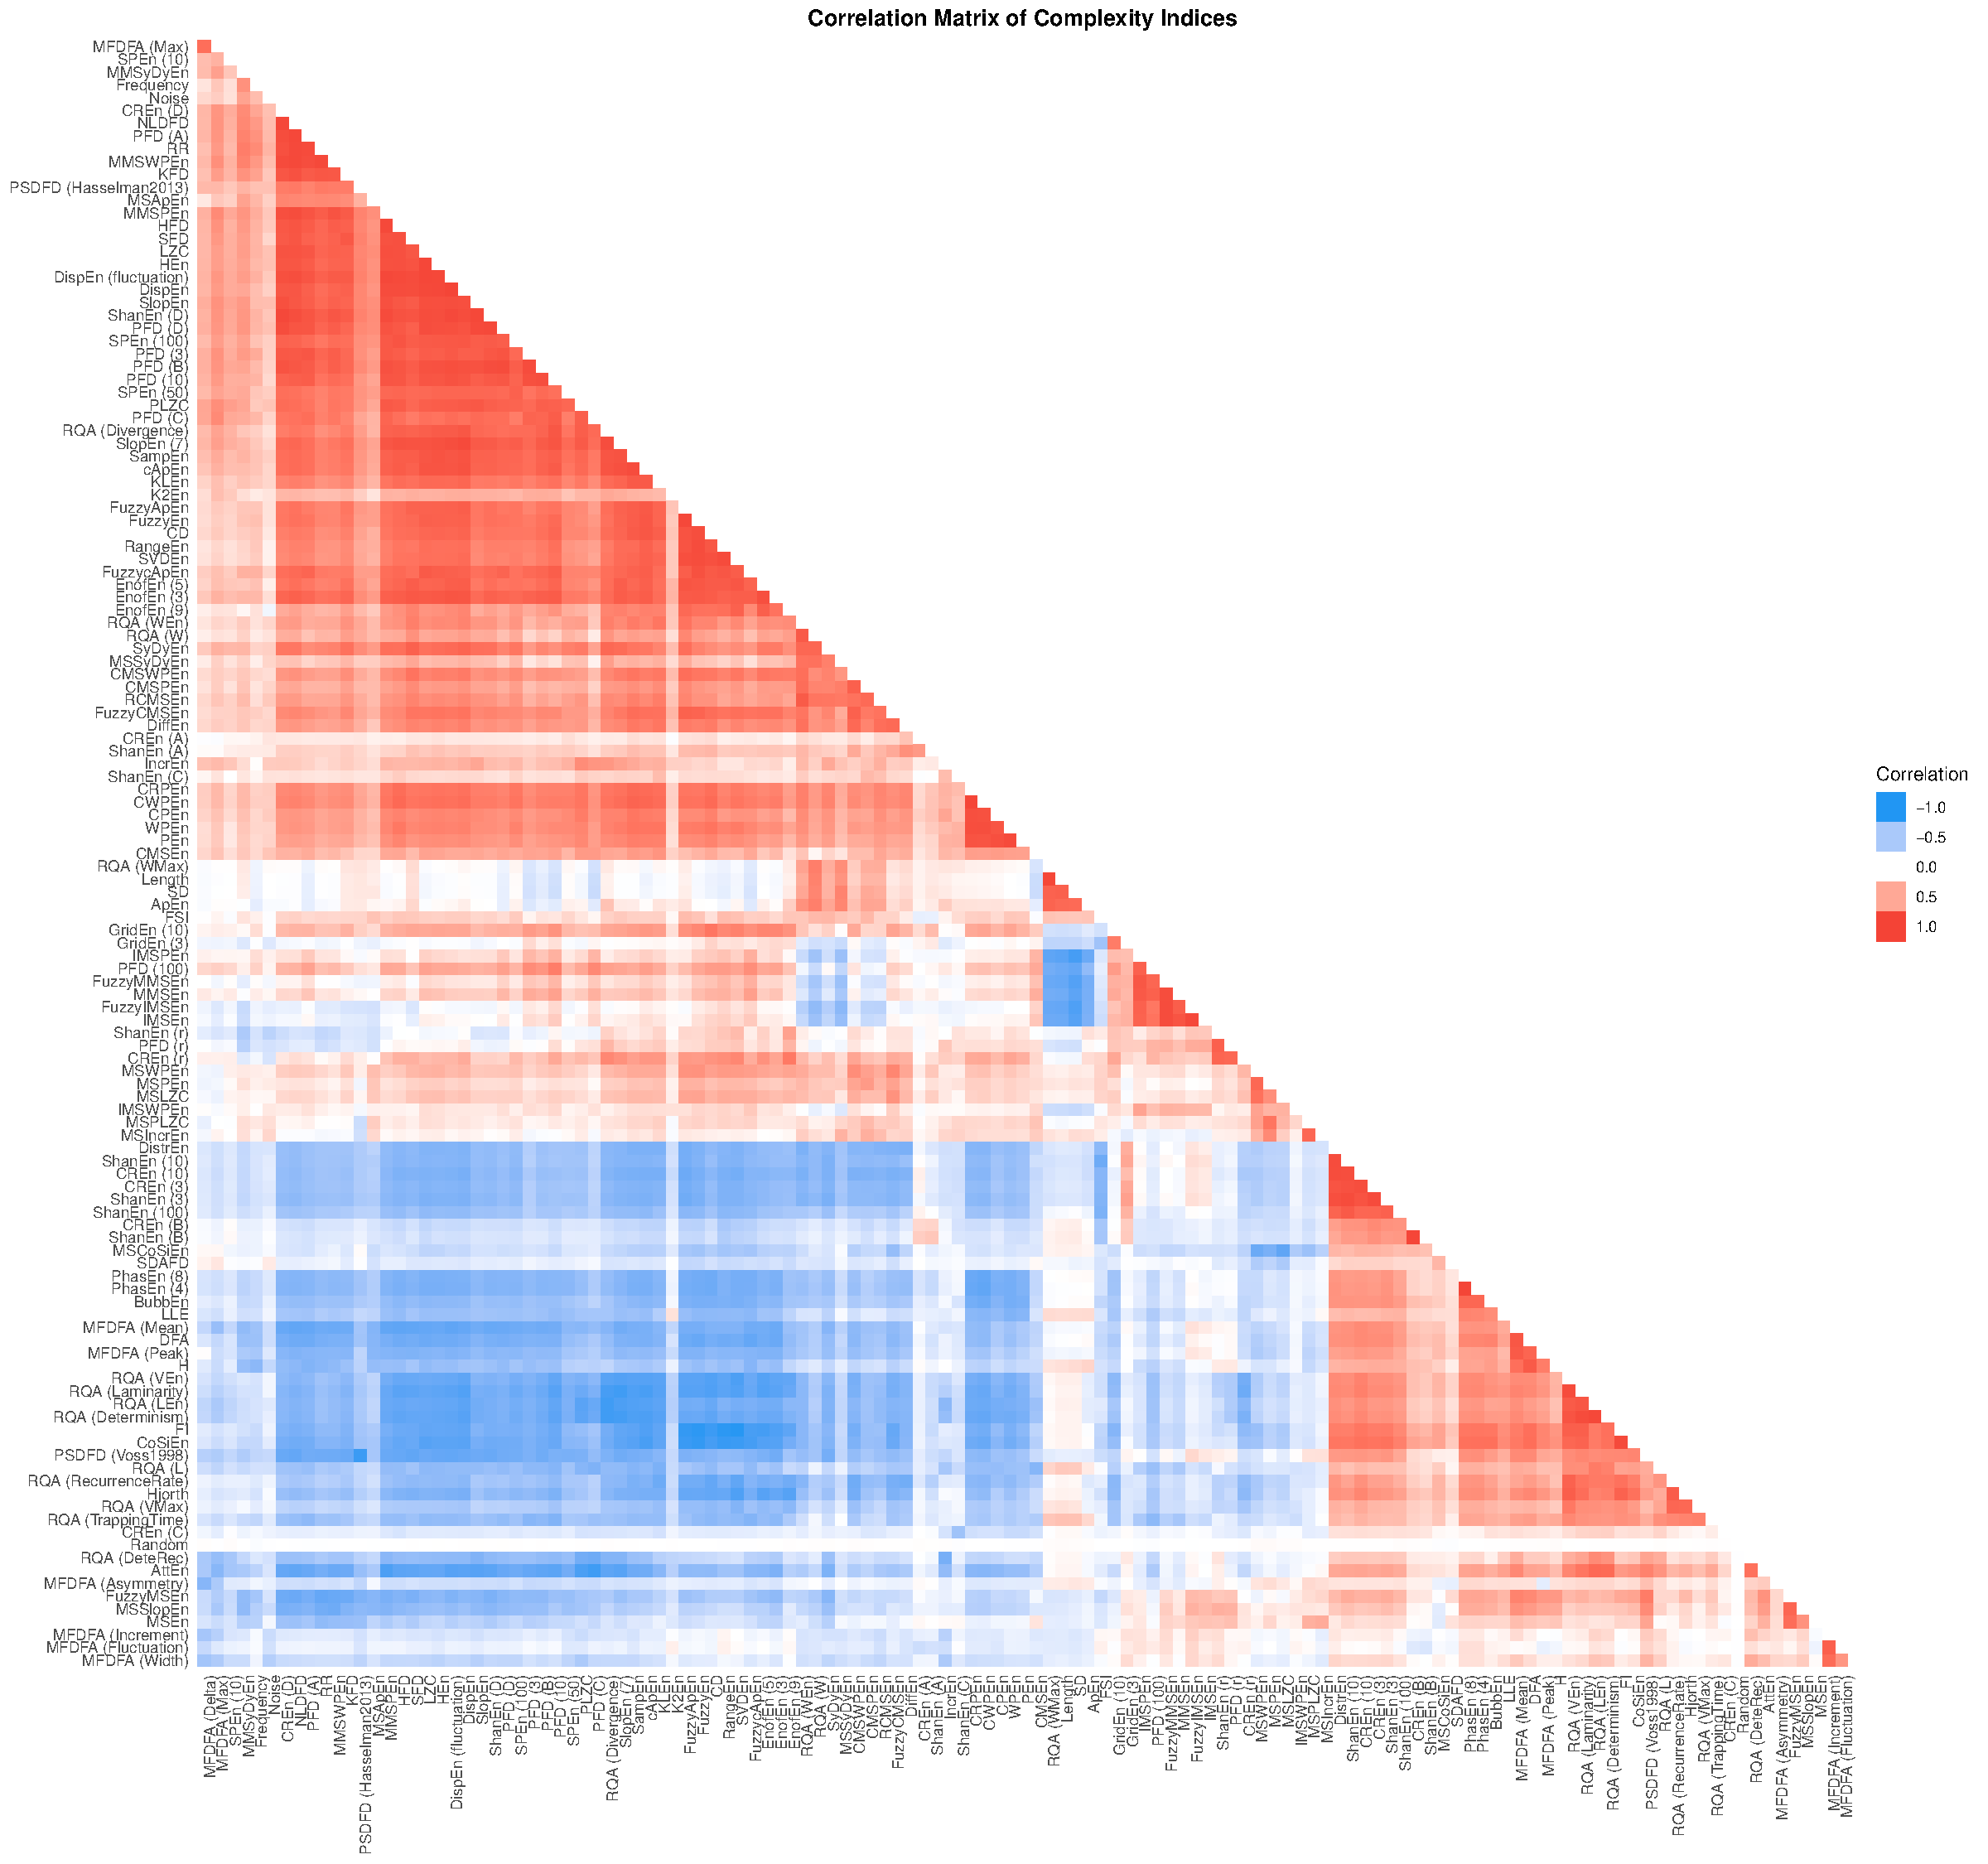
\includegraphics{manuscript_files/figure-latex/correlation-1.pdf}
\caption{\label{fig:correlation}Correlation Matrix.}
\end{figure}

The Pearson correlation analysis revealed that complexity indices, despite their multitude, their unicities and specificities, do indeed share similarities. They form clusters, with two major ones easily appearing to the naked eye (the blue and the red groups). These two anti-correlated groups are driven by the fact that some indices, by design, index the ``predictability'', whereas other the ``randomness'', and thus are negatively related to one-another (see \textbf{Figure 2}).

\hypertarget{factor-analysis}{%
\subsubsection{Factor Analysis}\label{factor-analysis}}

\begin{figure}
\centering
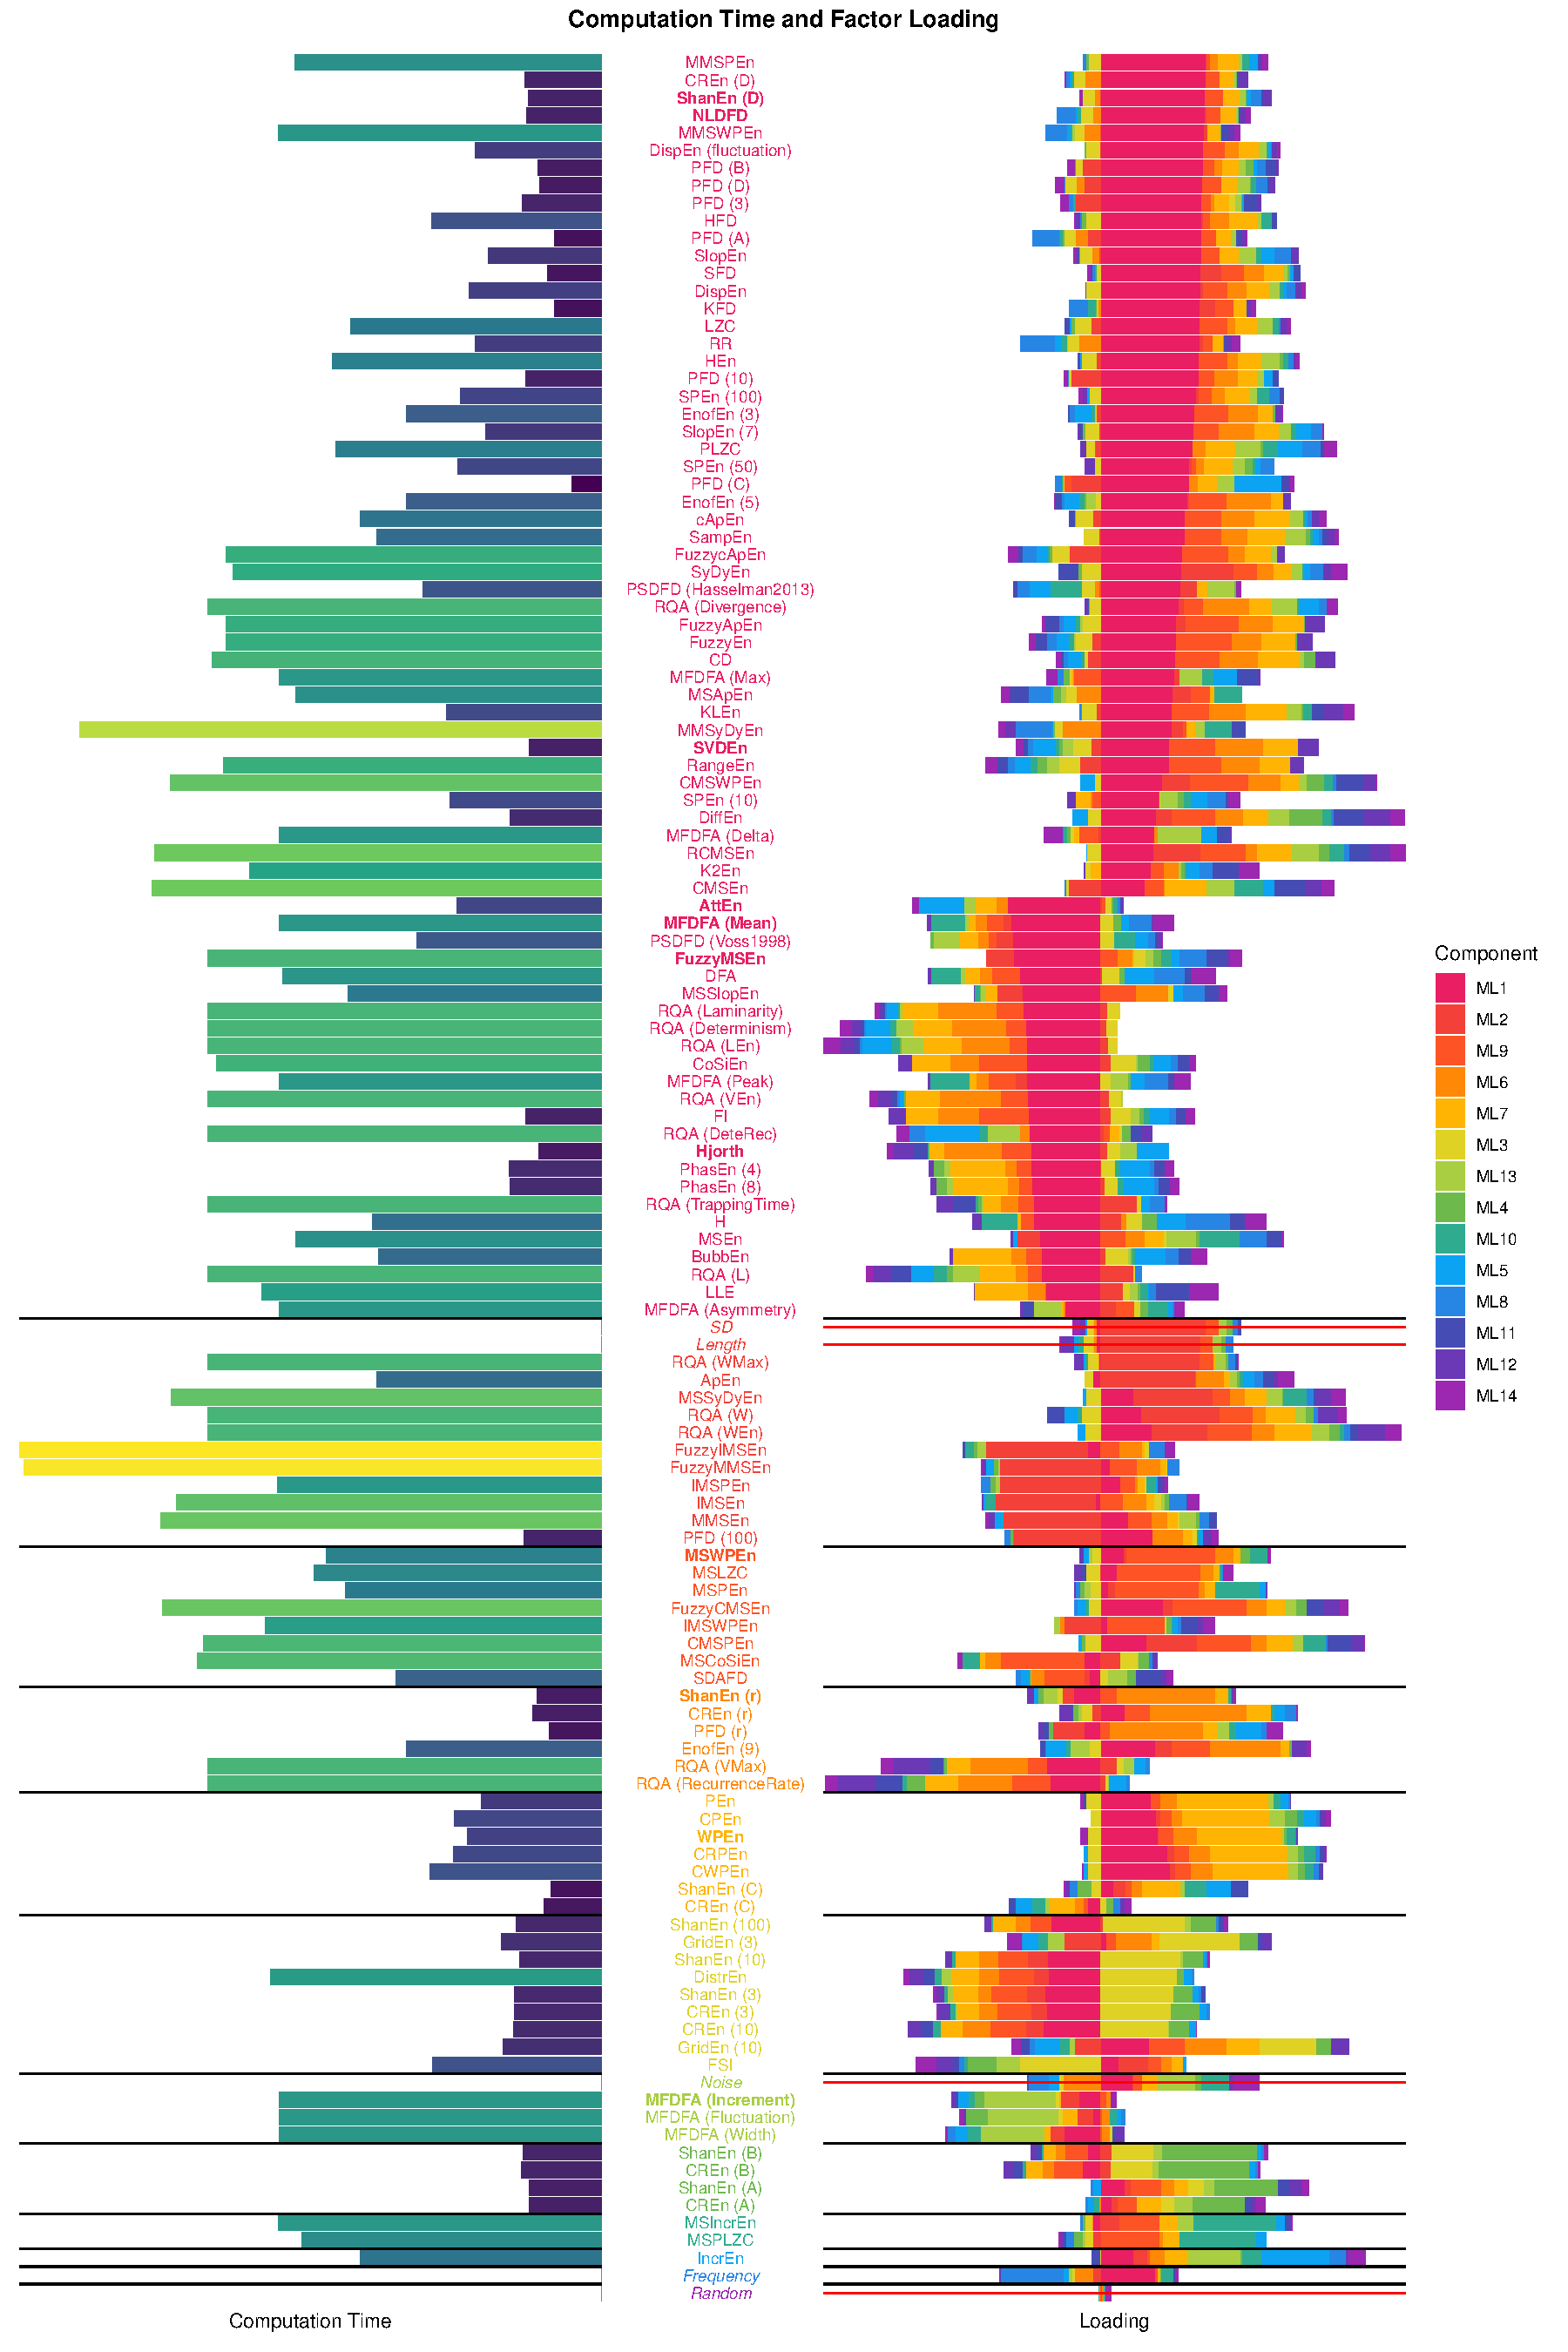
\includegraphics{manuscript_files/figure-latex/loadings-1.pdf}
\caption{\label{fig:loadings}Factor loadings and computation times of the complexity indices, colored by the factor they represent the most.}
\end{figure}

The agreement procedure for the optimal number of factors suggested that the 125 indices can be mapped on a multidimensional space of 14 orthogonal latent factors, that we extracted using a \emph{varimax} rotation. We then took interest in the loading profile of each indices, and in particular the latent dimension that maximally related to each index (see \textbf{Figure 3}).

The first factor is the closest to the largest amount of indices. Many indices with positive and strong loadings are particularly sensitive to the deviation of consecutive differences (e.g., \emph{ShanEn - D}, \emph{NLDFD}, \emph{PFD - D}). It was negatively loaded by indices related to Detrended Fluctuation Analysis (DFA), which tend to index the presence of long-term correlations. This latent factor might encapsulate the predominance of short-term vs.~long-term unpredictability. Indices that are the most representative (positively and negatively) and have a relatively low computational cost include \emph{ShanEn - D}, \emph{NLDFD}, \emph{PFD - D}, and \emph{AttEn}, \emph{PSDFD}, \emph{FuzzyMSEn}. The second factor was loaded maximally by signal \emph{length} and \emph{SD}, and thus might not capture features of complexity \emph{per se}. Indices the most related to it were indices known to be sensitive to signal length, such as \emph{ApEn}. The third factor included multiscale indices, such as \emph{MSWPEn}. The fourth factor included indices that quantified the diversity of the tendency of a signal to revisit a past state (within a certain tolerance threshold). It was positively loaded by \emph{ShanEn - r} and negatively by \emph{RQA - Reccurence Rate}. The fifth factor was loaded by permutation entropy indices, such as \emph{WPEn}. The sixth factor was driven by indices that were based on converting the signal into a number of bins. The seventh factor was loaded positively by the amount of noise, and negatively by multifractal indices such as \emph{MFDFA - Increment}, suggesting a sensitivity to regularity. The last notable result is that indices based on a symbolization (discretization) of the time series do tend to create factors alongside the symbolization method. Finally, as a manipulation check of our factorization method, the random vector does indeed form its own factor, and doesn't load unto anything else.

\hypertarget{correlation-network}{%
\subsubsection{Correlation Network}\label{correlation-network}}

For illustration purposes, we also represented the correlation matrix as a connectivity graph (see \textbf{Figure 4}).

\begin{figure}
\centering
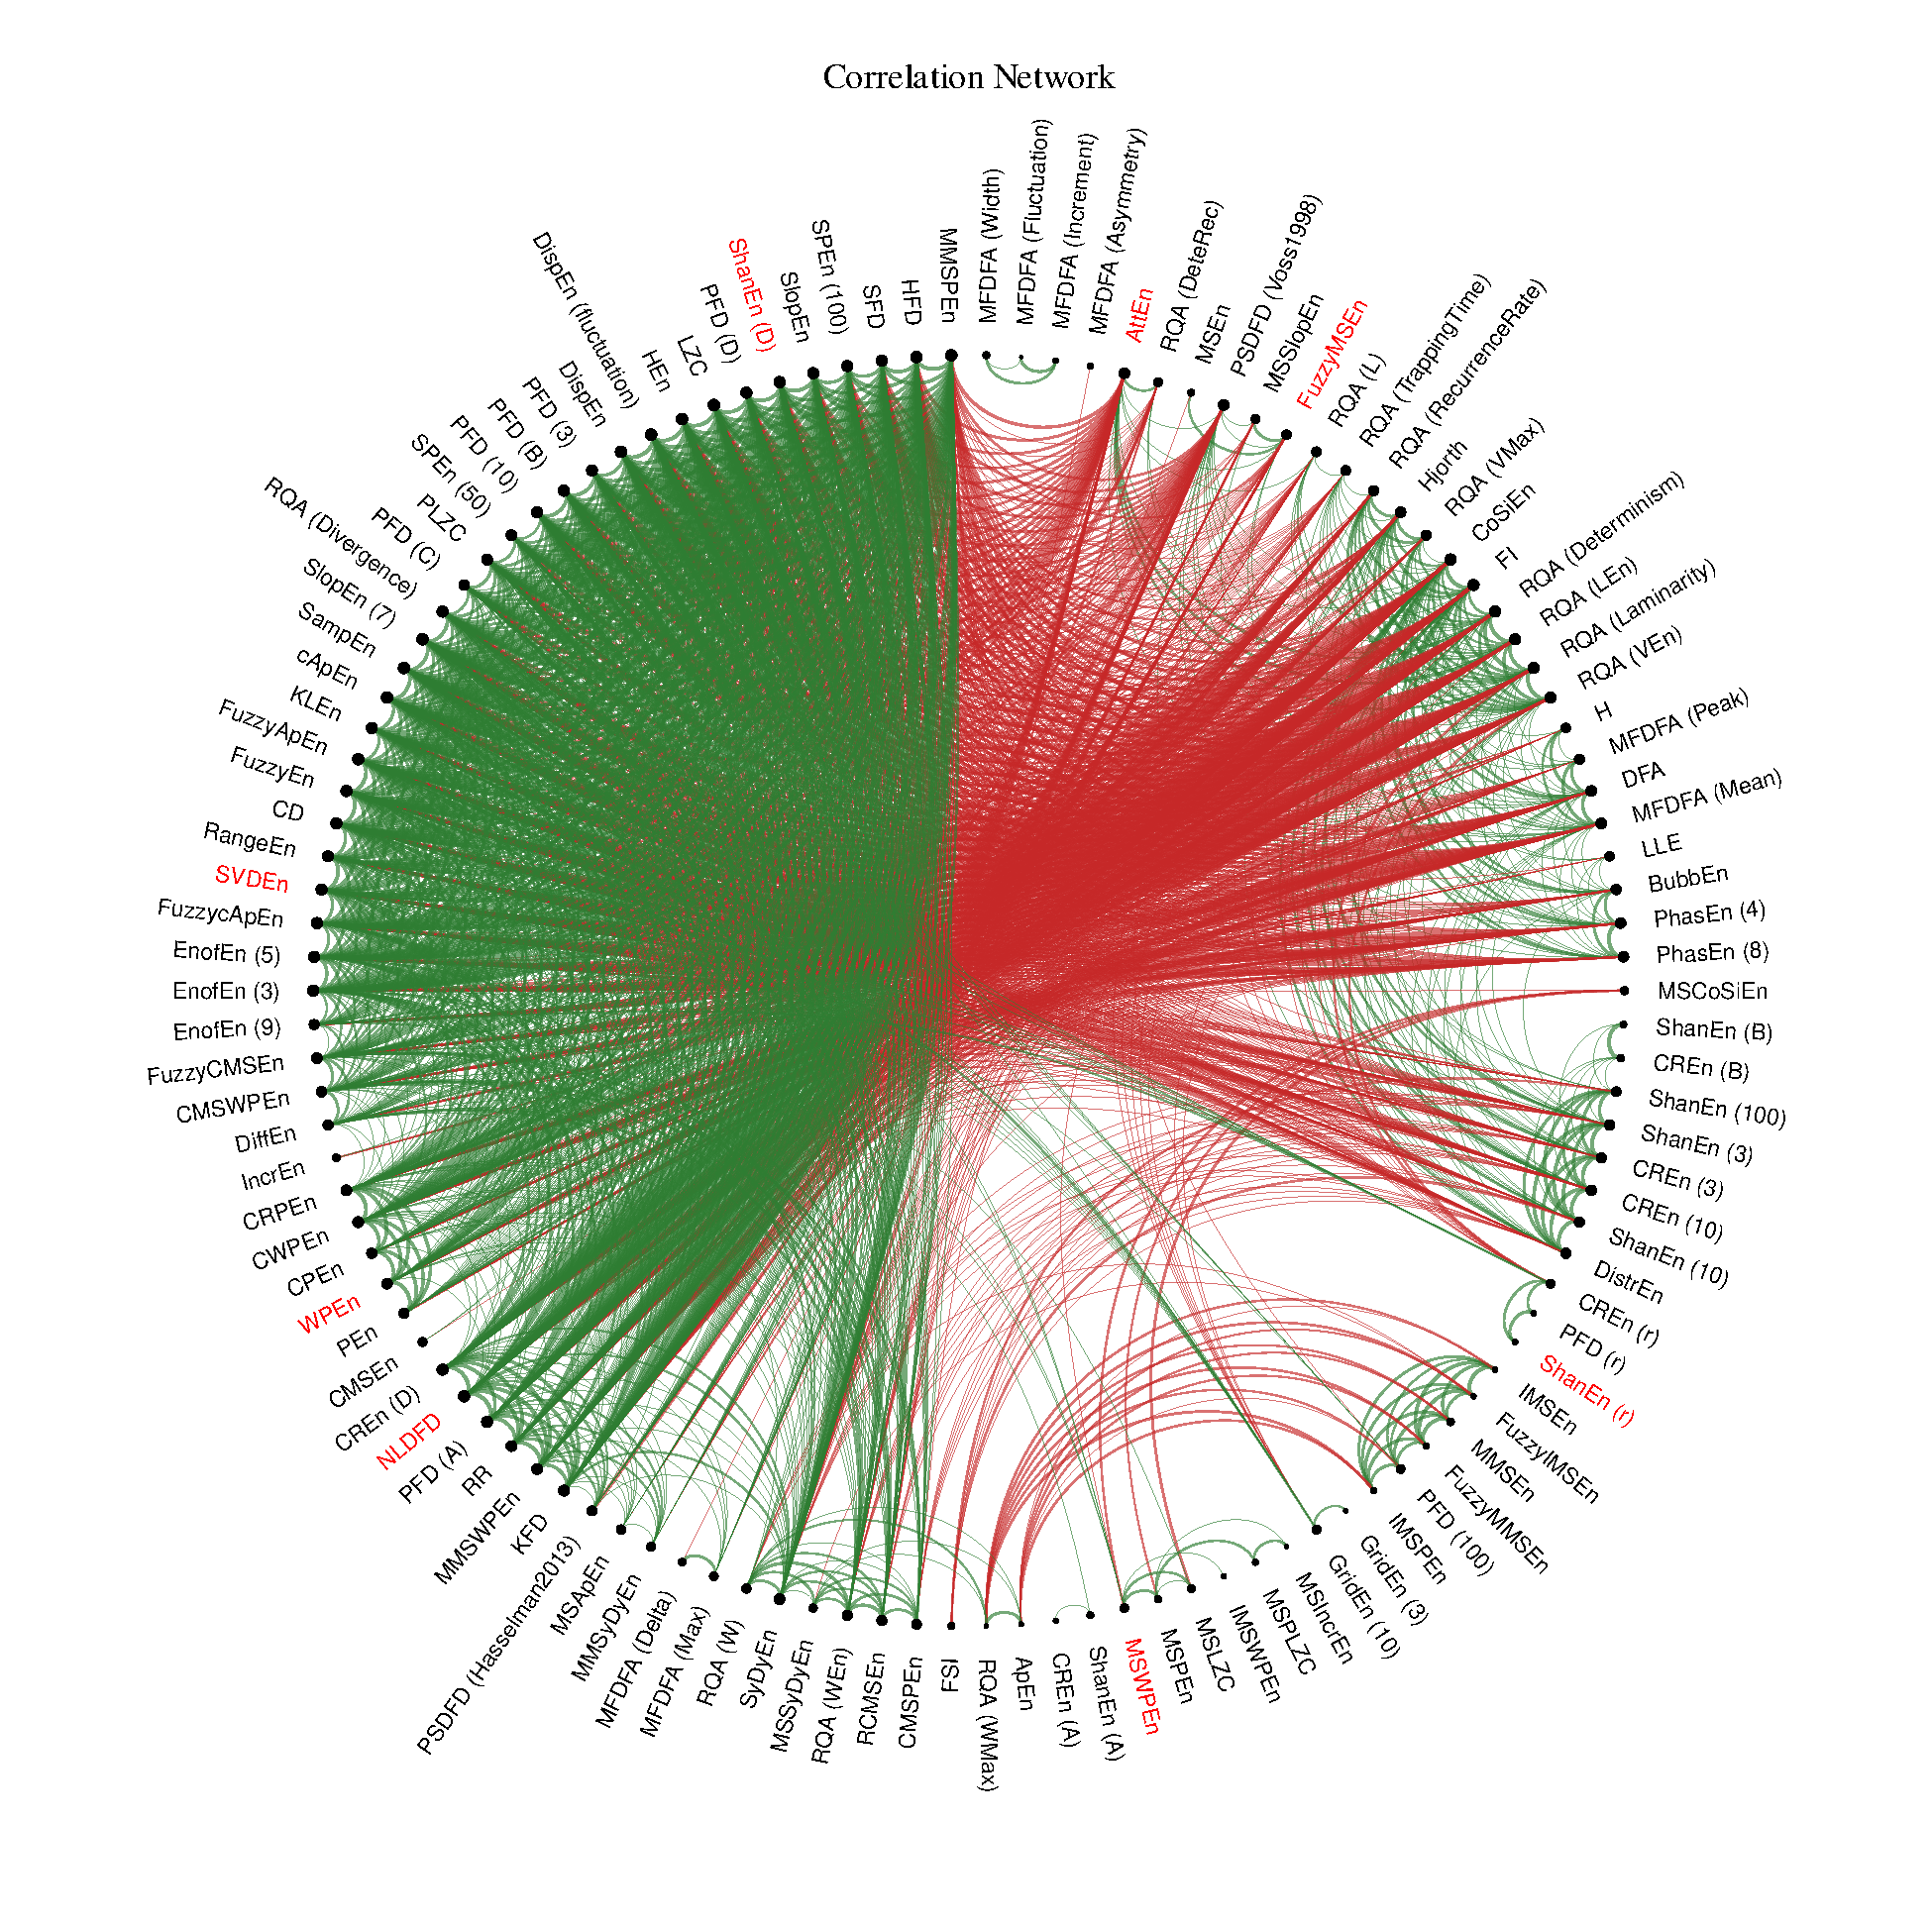
\includegraphics{manuscript_files/figure-latex/ggm-1.pdf}
\caption{\label{fig:ggm}Correlation network of the complexity indices. Only the links where \textbar r\textbar{} \textgreater{} 0.6 are displayed.}
\end{figure}

\hypertarget{hierarchical-clustering}{%
\subsubsection{Hierarchical Clustering}\label{hierarchical-clustering}}

We ran hierarchical clustering (with a Ward D2 distance) to provide additional information or confirmation about the groups discussed above. This allowed us to fine-grain our recommendations of complimentary complexity indices (see \textbf{Figure 5}).

\begin{figure}
\centering
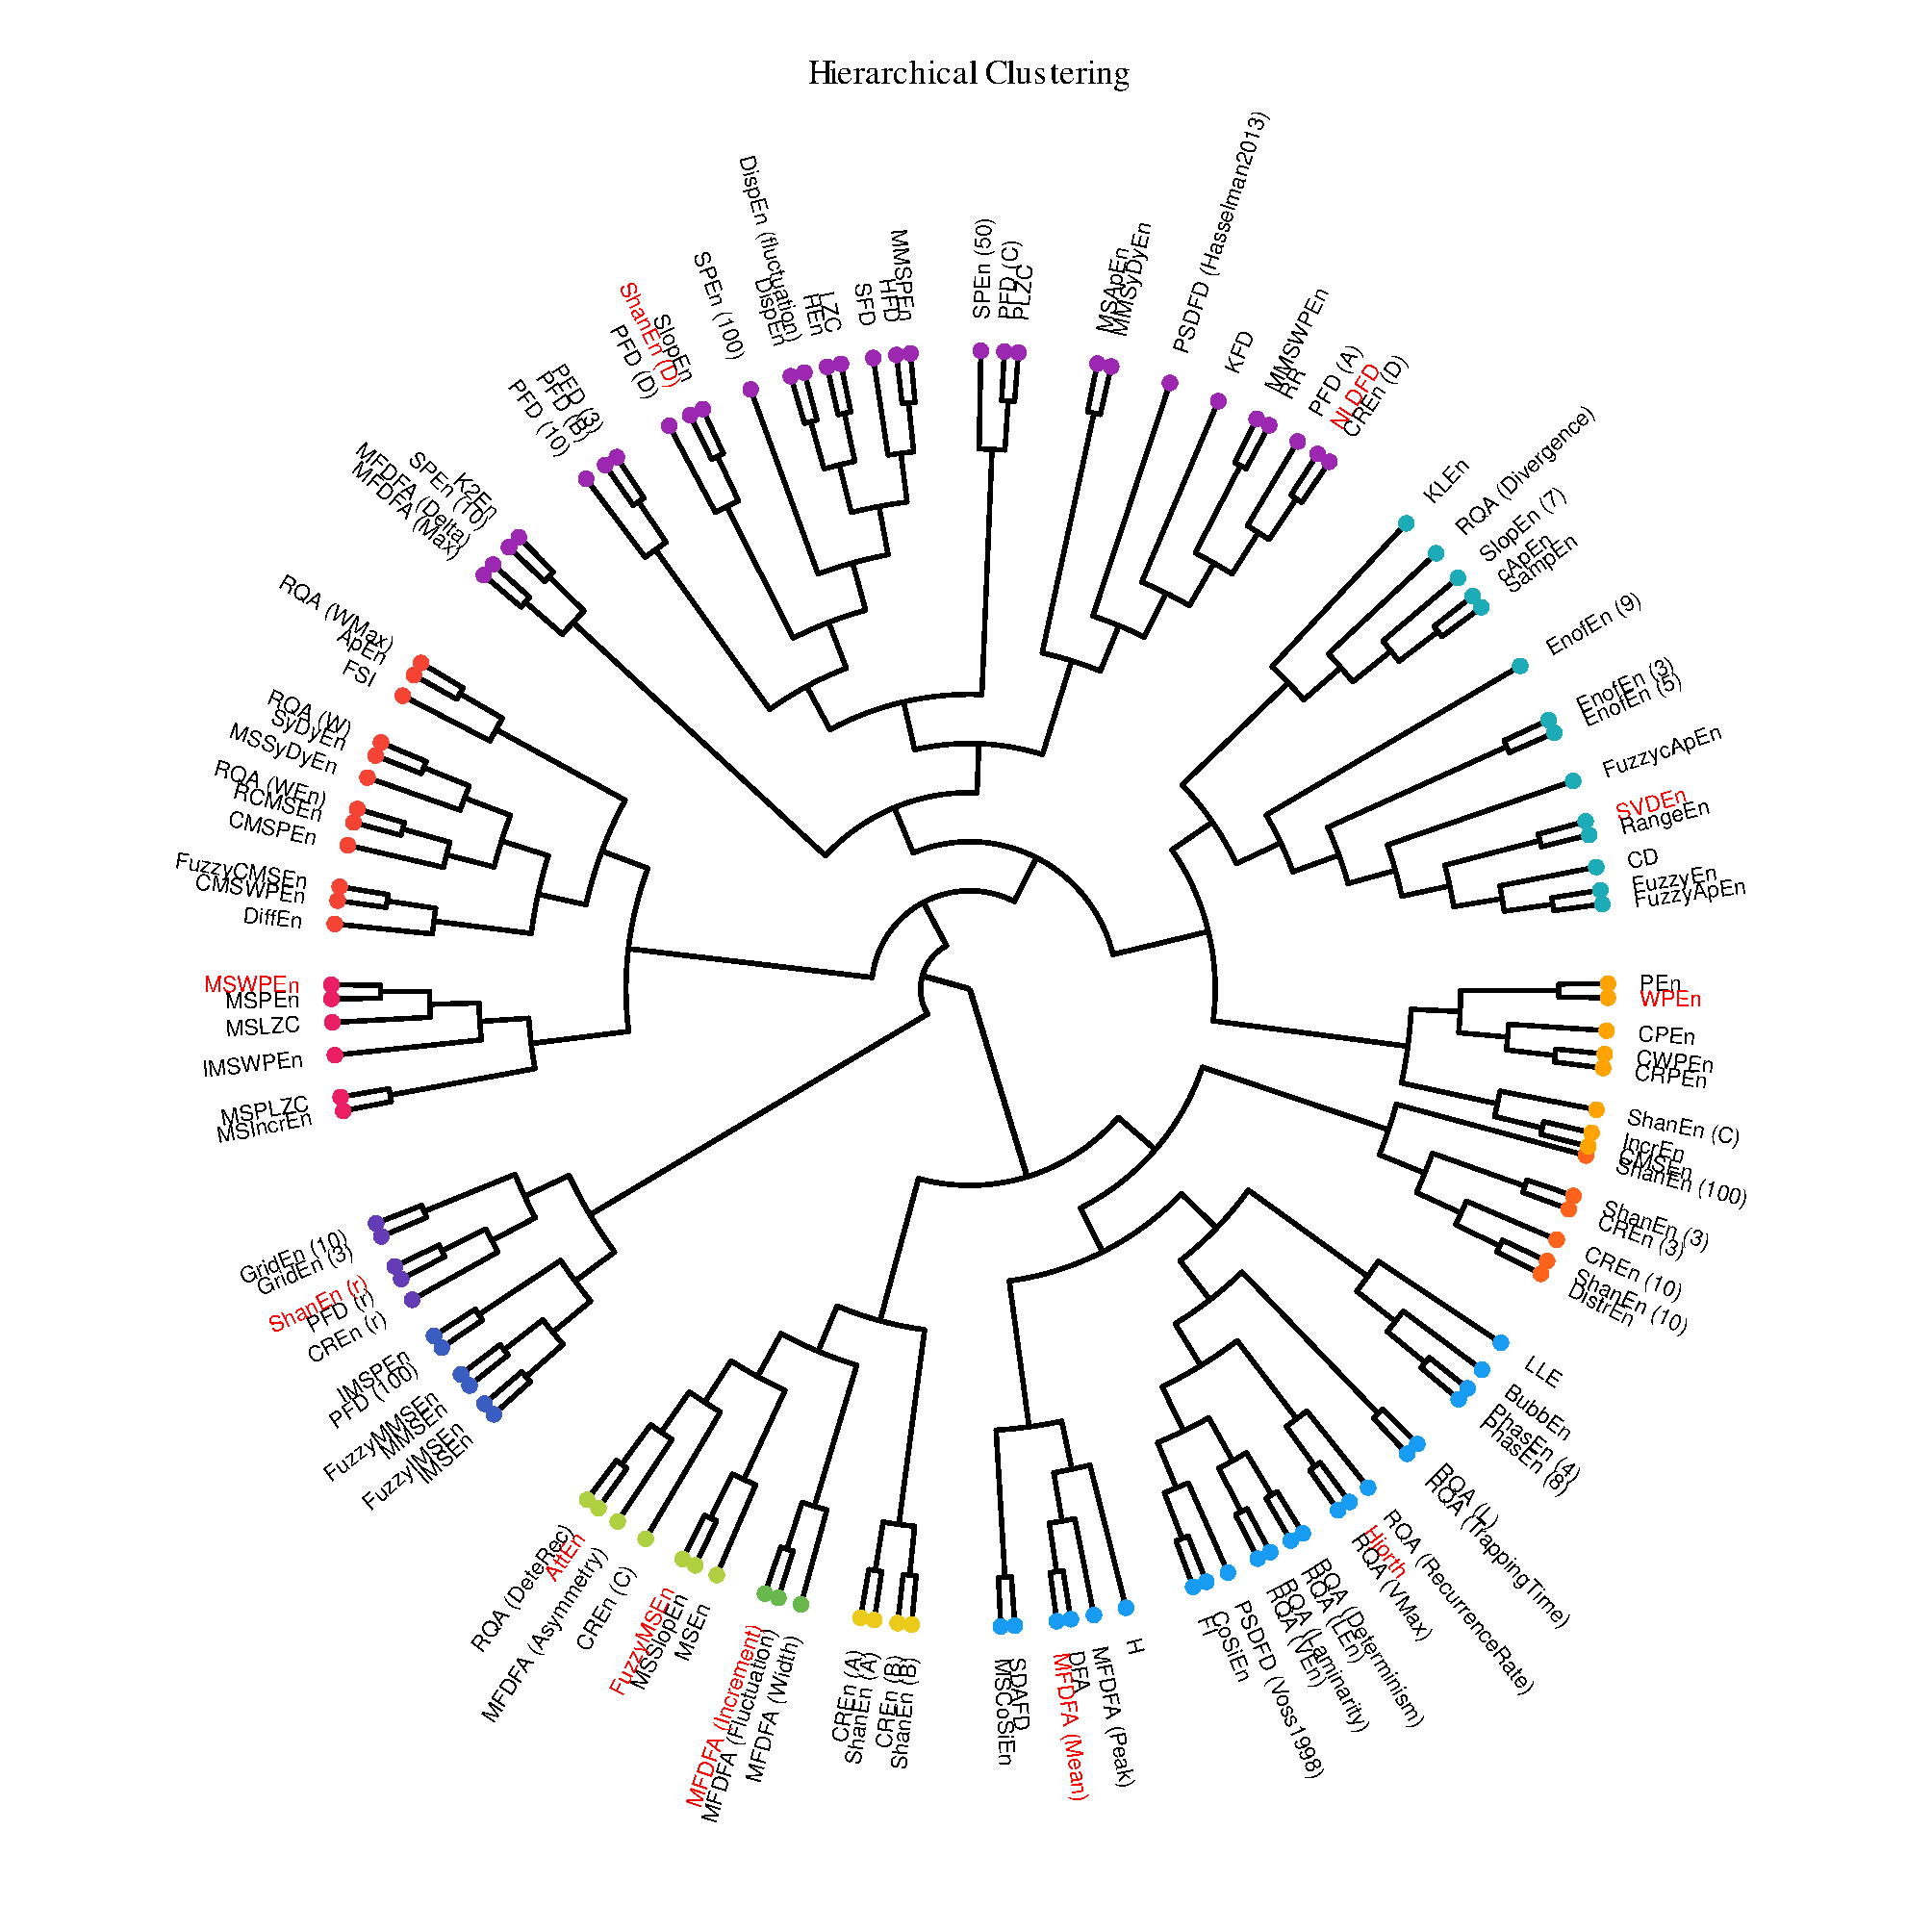
\includegraphics{manuscript_files/figure-latex/clustering-1.pdf}
\caption{\label{fig:clustering}Dendrogram representing the hierarchical clustering of the complexity indices.}
\end{figure}

\hypertarget{discussion}{%
\subsection{Discussion}\label{discussion}}

As complexity science grows in size and application, a systematic approach to compare their ``performance'' becomes necessary to increase the clarity and structure of the field. The word \emph{performance} is here to be understood in a relative sense, as any such endeavor faces the ``hard problem'' of complexity science. The indices are sensitive to specific objective properties of a signal that we consider part of over-arching concepts such as ``complex'' and ``chaotic''. But it is unclear how these high-level concepts transfer back, in a top-down fashion, into a combination of lower-level features, such as short-term vs.~long-term variability, auto-correlation, information, randomness, and so on. As such, it is conceptually complicated to benchmark complexity measures against ``objectively'' complex vs.~non-complex signals. In other words, we know that different characteristics can contribute to the ``complexity'' of a signal, but there is not a one-to-one correspondence between the latter and the former.

Hence the choice of the current paradigm, in which we generated different types of signals to which we systematically added different types and amount of perturbations. However, we did not seek at measuring how complexity indices can discriminate between these features or systems, nor did we attempt at mimicking real-life signals or scenarios. The goal was instead to generate enough variability to reliably map the relationships between the indices.

The plurality of underlying components of empirical complexity (what is measured by complexity indices) seems to be somewhat confirmed by our results, showing that complexity indices are more or less sensitive to various orthogonal latent dimensions. One of the limitation of the current study has to do with the limited possibilities of interpretation of these underlying dimensions, and future studies are needed to discuss them.

Indices that were highlighted as encapsulating information about different underlying dimensions at a relatively low computational cost include \emph{ShanEn (D)}, \emph{NLDFD}, \emph{SVDEn}, \emph{AttEn}, \emph{PSDFD}, \emph{MFDFA (Mean)}, \emph{FuzzyMSEn}, \emph{MSWPEn}, \emph{MFDFA (Increment)}, \emph{ShanEn (r)}, \emph{Hjorth} and \emph{WPEn}. These indices might be complimentary in offering a comprehensive profile of the complexity of a time series. Future studies are needed to analyze the nature of the dominant sensitivities of group of indices, so that results can be more easily interpreted and integrated into new studies and novel theories.

\newpage

\hypertarget{references}{%
\section{References}\label{references}}

\hypertarget{refs}{}
\begin{CSLReferences}{1}{0}
\leavevmode\vadjust pre{\hypertarget{ref-bassingthwaighte2013fractal}{}}%
Bassingthwaighte, J. B., Liebovitch, L. S., \& West, B. J. (2013). \emph{Fractal physiology}. Springer.

\leavevmode\vadjust pre{\hypertarget{ref-ehlers1995chaos}{}}%
Ehlers, C. L. (1995). Chaos and complexity: Can it help us to understand mood and behavior? \emph{Archives of General Psychiatry}, \emph{52}(11), 960--964.

\leavevmode\vadjust pre{\hypertarget{ref-lau2021brain}{}}%
Lau, Z. J., Pham, T., Annabel, S., \& Makowski, D. (2021). \emph{Brain entropy, fractal dimensions and predictability: A review of complexity measures for EEG in healthy and neuropsychiatric populations}.

\leavevmode\vadjust pre{\hypertarget{ref-parametersArticle}{}}%
Lüdecke, D., Ben-Shachar, M., Patil, I., \& Makowski, D. (2020). Extracting, computing and exploring the parameters of statistical models using {R}. \emph{Journal of Open Source Software}, \emph{5}(53), 2445. \url{https://doi.org/10.21105/joss.02445}

\leavevmode\vadjust pre{\hypertarget{ref-seeArticle}{}}%
Lüdecke, D., Patil, I., Ben-Shachar, M. S., Wiernik, B. M., Waggoner, P., \& Makowski, D. (2021). {see}: An {R} package for visualizing statistical models. \emph{Journal of Open Source Software}, \emph{6}(64), 3393. \url{https://doi.org/10.21105/joss.03393}

\leavevmode\vadjust pre{\hypertarget{ref-correlationArticle}{}}%
Makowski, D., Ben-Shachar, M., Patil, I., \& Lüdecke, D. (2020). Methods and algorithms for correlation analysis in {R}. \emph{Journal of Open Source Software}, \emph{5}(51), 2306. \url{https://doi.org/10.21105/joss.02306}

\leavevmode\vadjust pre{\hypertarget{ref-modelbasedPackage}{}}%
Makowski, D., Lüdecke, D., Ben-Shachar, M. S., \& Patil, I. (2022). \emph{{modelbased}: Estimation of model-based predictions, contrasts and means} (Version 0.7.2.1) {[}Computer software{]}. \url{https://CRAN.R-project.org/package=modelbased} (Original work published 2020)

\leavevmode\vadjust pre{\hypertarget{ref-Makowski2021neurokit}{}}%
Makowski, D., Pham, T., Lau, Z. J., Brammer, J. C., Lespinasse, F., Pham, H., Schölzel, C., \& Chen, S. H. A. (2021). {NeuroKit}2: A python toolbox for neurophysiological signal processing. \emph{Behavior Research Methods}, \emph{53}(4), 1689--1696. \url{https://doi.org/10.3758/s13428-020-01516-y}

\end{CSLReferences}


\clearpage
\renewcommand{\listfigurename}{Figure captions}


\end{document}
